%-B--------------------------------------------------------------------------B-%
\begin{frame}[allowframebreaks]
\frametitle{Définitions}

\begin{block}{Corpus}

Un \textbf{corpus} est un ensemble de documents (textes, images, vidéos, etc.) 
regroupés dans une optique précise.\\[0.5em]

Dans le cadre de ce cours~: \alert{\fbox{corpus $\to$ corpus de textes}}\\[0.5em]

Plusieurs caractéristiques sont à prendre en compte pour la création d'un corpus
bien formé~:

	\begin{itemize}
		\item la taille;
		\item le langage;
		\item le temps couvert par les textes du corpus;
		\item le registre de langage.
	\end{itemize}

\end{block}

Source~: \url{http://fr.wikipedia.org/wiki/Corpus}

\framebreak

\begin{block}{Taille}

Le corpus doit évidemment atteindre une taille critique pour permettre des 
traitements statistiques fiables.

    \begin{itemize}
        \item Si le corpus est utilisé pour construire des modèles de langue, quelle 
              doit être sa taille minimum~? 1M mots, 10M mots, etc.
    \end{itemize}

\end{block}

\begin{block}{Langage}

Un corpus \textbf{monolingue} bien formé doit nécessairement couvrir une seule 
langue, et une seule déclinaison de cette langue (e.g.~français de France et 
français du Québec).

\end{block}

\framebreak

\begin{block}{Période couverte}

Le temps joue un rôle important dans l'évolution du langage~: le français parlé 
aujourd'hui ne ressemble pas au français parlé il y a 200 ans ni, de façon plus 
subtile, au français parlé il y a 10 ans, à cause notamment des néologismes.

\end{block}


\begin{block}{Registre de langage}

Un corpus construit à partir de textes scientifiques ne peut être utilisé pour 
extraire des informations sur les textes vulgarisés, et un corpus mélangeant des
textes scientifiques et vulgarisés ne permettra pas de tirer de conclusion sur 
ces deux registres.

\end{block}

\end{frame}
%-E--------------------------------------------------------------------------E-%

%-B--------------------------------------------------------------------------B-%
\begin{frame}
\frametitle{Corpus parallèle}

Un corpus parallèle est un ensemble de paires de textes tel que, pour une 
paire, un des textes est la traduction de l'autre. \\[0.5em]

Construire un corpus parallèle nécessite un \textbf{alignement} des unités 
textuelles~:

    \begin{itemize}
        \item mettre en correspondance des unités textuelles en langue source
              avec celles de la langue cible.
    \end{itemize}

L'alignement des unités textuelles peut être manuel ou automatique.\\[0.5em]

La granularité de l'alignement (documents, phrases, mots) dépend de 
l'utilisation du corpus~:

    \begin{itemize}
        \item traduction automatique, génération de paraphrases, construction
              dictionnaires bilingues, etc.
    \end{itemize}

\end{frame}
%-E--------------------------------------------------------------------------E-%

%-B--------------------------------------------------------------------------B-%
\begin{frame}
\frametitle{Alignement de phrases}

\begin{columns}[c] 
    \small

    \column{.45\textwidth}

    Il s'agit de l'un des sauropodes les plus connus. \\[0.5em]

    C'était un très grand quadrupède au long cou, avec une longue queue en 
    forme de fouet.\\[0.5em]

    Ses membres antérieurs étaient légèrement plus courts que ses membres 
    postérieurs, ce qui lui donnait une posture horizontale.\\[1.2em]
    ~

    \column{.1\textwidth}

    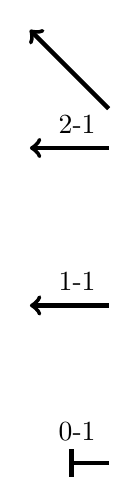
\begin{tikzpicture}
        \draw [ultra thick, <-] (0,5.5) -- (1,4.5);
        \draw [ultra thick, <-] (0,4) -- (1,4);
        \node at (0.6,4.3) {2-1};
        \draw [ultra thick, <-] (0,2) -- (1,2);
        \node at (0.6,2.3) {1-1};
        \draw [ultra thick,|-] (0.5,0) -- (1,0);
        \node at (0.6,0.4) {0-1};
    \end{tikzpicture}
    \vspace*{1em}

    \column{.45\textwidth}

    One of the best-known sauropods, Diplodocus was a very large long-necked 
    quadrupedal animal, with a long, whip-like tail.\\[1.2em]

    Its forelimbs were slightly shorter than its hind limbs, resulting in a 
    largely horizontal posture.\\[1.2em]

    It is the longest dinosaur known from a complete skeleton.

\end{columns}

\vspace*{1em}

Source~: \url{http://en.wikipedia.org/wiki/Diplodocus}

\end{frame}
%-E--------------------------------------------------------------------------E-%


%-B--------------------------------------------------------------------------B-%
\begin{frame}
\frametitle{Alignement de mots}

Exemple d'alignment simple.

\begin{center}
Je suis Français . \\
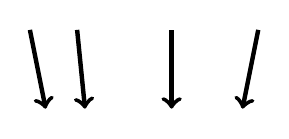
\begin{tikzpicture}
    \draw [ultra thick, <-] (0.4,0) -- (0.2,1);
    \draw [ultra thick, <-] (0.9,0) -- (0.8,1);
    \draw [ultra thick, <-] (2,0) -- (2,1);
    \draw [ultra thick, <-] (2.9,0) -- (3.1,1);
\end{tikzpicture}\\[-0.2em]
I am French .
\end{center}

\vspace*{1em}

Exemple d'alignment plus compliqué.

\begin{center}
Je m' appelle Paul . \\
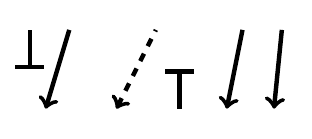
\begin{tikzpicture}
    \draw [ultra thick, |-] (0.4,0.5) -- (0.4,1);
    \draw [ultra thick, <-] (0.6,0) -- (0.9,1);
    \draw [dashed, ultra thick, <-] (1.5,0) -- (2,1);
    \draw [ultra thick, -|] (2.3,0) -- (2.3,0.5);
    \draw [ultra thick, <-] (2.9,0) -- (3.1,1);
    \draw [ultra thick, <-] (3.5,0) -- (3.6,1);
\end{tikzpicture}\\[-0.2em]
My name is Paul .
\end{center}

\end{frame}
%-E--------------------------------------------------------------------------E-%

%-B--------------------------------------------------------------------------B-%
\begin{frame}
\frametitle{Corpora parallèles disponibles}

\begin{itemize}
    \item Europarl \\
    Délibérations du Parlement européen disponibles en 21 langues.
    \item OpenSubtitles\\
    Sous-titres de films disponibles en 30 langues.
    \item Hansard (Canada)\\
    Rranscriptions officielles des débats parlementaires dans les gouvernements.
\end{itemize}


\end{frame}
%-E--------------------------------------------------------------------------E-%



%-B--------------------------------------------------------------------------B-%
\begin{frame}
\frametitle{}

\end{frame}
%-E--------------------------------------------------------------------------E-%

